\documentclass[10pt,letterpaper]{article}
\usepackage{multicol}
\usepackage{calc}
\usepackage{ifthen}
\usepackage[landscape]{geometry}
\usepackage{hyperref}
\usepackage{amsmath}
\usepackage{graphicx}

% To make this come out properly in landscape mode, do one of the following
% 1.
%  pdflatex latexsheet.tex
%
% 2.
%  latex latexsheet.tex
%  dvips -P pdf  -t landscape latexsheet.dvi
%  ps2pdf latexsheet.ps


% If you're reading this, be prepared for confusion.  Making this was
% a learning experience for me, and it shows.  Much of the placement
% was hacked in; if you make it better, let me know...


% 2008-04
% Changed page margin code to use the geometry package. Also added code for
% conditional page margins, depending on paper size. Thanks to Uwe Ziegenhagen
% for the suggestions.

% 2006-08
% Made changes based on suggestions from Gene Cooperman. <gene at ccs.neu.edu>


% To Do:
% \listoffigures \listoftables
% \setcounter{secnumdepth}{0}


% This sets page margins to .5 inch if using letter paper, and to 1cm
% if using A4 paper. (This probably isn't strictly necessary.)
% If using another size paper, use default 1cm margins.
\ifthenelse{\lengthtest { \paperwidth = 11in}}
	{ \geometry{top=.5in,left=.5in,right=.5in,bottom=.5in} }
	{\ifthenelse{ \lengthtest{ \paperwidth = 297mm}}
		{\geometry{top=1cm,left=1cm,right=1cm,bottom=1cm} }
		{\geometry{top=1cm,left=1cm,right=1cm,bottom=1cm} }
	}

% Turn off header and footer
\pagestyle{empty}
 

% Redefine section commands to use less space
\makeatletter
\renewcommand{\section}{\@startsection{section}{1}{0mm}%
                                {-1ex plus -.5ex minus -.2ex}%
                                {0.5ex plus .2ex}%x
                                {\normalfont\large\bfseries}}
\renewcommand{\subsection}{\@startsection{subsection}{2}{0mm}%
                                {-1explus -.5ex minus -.2ex}%
                                {0.5ex plus .2ex}%
                                {\normalfont\normalsize\bfseries}}
\renewcommand{\subsubsection}{\@startsection{subsubsection}{3}{0mm}%
                                {-1ex plus -.5ex minus -.2ex}%
                                {1ex plus .2ex}%
                                {\normalfont\small\bfseries}}
\makeatother

% Define BibTeX command
\def\BibTeX{{\rm B\kern-.05em{\sc i\kern-.025em b}\kern-.08em
    T\kern-.1667em\lower.7ex\hbox{E}\kern-.125emX}}

% Don't print section numbers
\setcounter{secnumdepth}{0}


\setlength{\parindent}{0pt}
\setlength{\parskip}{0pt plus 0.5ex}

\DeclareMathOperator*{\argmin}{arg\,min}
\DeclareMathOperator*{\argmax}{arg\,max}


% -----------------------------------------------------------------------

\begin{document}

\raggedright
\footnotesize
\begin{multicols}{3}


% multicol parameters
% These lengths are set only within the two main columns
%\setlength{\columnseprule}{0.25pt}
\setlength{\premulticols}{1pt}
\setlength{\postmulticols}{1pt}
\setlength{\multicolsep}{1pt}
\setlength{\columnsep}{2pt}

\begin{center}
     \Large{\textbf{Machine Learning Cheat Sheet}} \\
\end{center}

\section{Estimating Parameters}

\subsection{Likelihood of $\theta$ given the sample D}

\begin{equation*}
l(\theta | D) = p(D | \theta) = \prod_t p(x^t | \theta)
\end{equation*}

\subsection{Log likelihood}
\begin{equation*}
L(\theta | D) = \log l(\theta | D) = \sum_t \log p(x^t | \theta)
\end{equation*}

\subsection{Maximum Likelihood Estimation (MLE)}

\begin{equation*}
	\theta_{MLE} = \underset{\theta}{\argmax} \ L(\theta | D)
\end{equation*}

\subsection{Bernoulli}
\begin{equation*}
P(x) = p_0^x(1-p_0)^{(1-x)}
\end{equation*}
\begin{equation*}
L(p_0 | D) = \log \prod_t p_0^{x^t}(1-p_0)^{(1-x^t)}
\end{equation*}
\begin{equation*}
MLE: p_0 = \sum_t x^t / N
\end{equation*}
\begin{align*}
\theta_{MLE} &= \argmax_{\theta} L(p_0 | D) \\ 
&= \argmax_{\theta} \log \prod_t p_0^{x^t}(1-p_0)^{(1-x^t)} \\
&= \argmax_{\theta} \sum_t \log p_0^{x^t}(1-p_0)^{(1-x^t)} \\
&= \argmax_{\theta} \sum_t [x^t \log p_0 + (1 - x^t) \log(1 - p_0)]
\end{align*}
\begin{align*}
\frac{\partial L(p_0|D)}{\partial p_0} &= 0 \\
\frac{\partial L(p_0|D)}{\partial p_0} &=
\frac{\sum_t x^t}{p_0} + \frac{\sum_t (1 - x^t)}{(1 - p_0)} = 0 \\
(\sum_{i=1}^{n} x_i) \cdot (1 - \theta) &= \theta \cdot \sum_{i=1}^{n} (1-x_i) \\ 
\sum_{t} x^t - \theta \cdot \sum_{t} &= \theta \cdot \sum_{t} (1-x^t) \\ 
\theta = \frac{\sum_{t} x^t}{\sum_{t} x^t + \sum_{t} (1-x^t)} &= \frac{n_1}{n}
\end{align*}

\subsection{Gaussian (Normal)}

\begin{align*}
p(\theta) &= \frac{1}{\sqrt{2 \pi} \sigma_1} e ^{-\frac{(\theta - \mu_1)^2}{2 \sigma_1^2}} \\
p(x | \theta) &= \frac{1}{\sqrt{2 \pi} \sigma_2} e ^{-\frac{(x - \theta)^2}{2 \sigma_2^2}} \\
\theta_{MLE} &= \argmax_{\theta} p(\theta | D ) = \argmax_{\theta} p(D |\theta) p(\theta) \\
&= \argmax_{\theta} \log(p(D |\theta) p(\theta)) \\
&= \argmax_{\theta} \log p(D |\theta) + \log p(\theta) \\
\end{align*}
\begin{align*}
&= \argmax (- \frac{1}{2} \log 2 \pi \sigma_2^2 - \frac{(x-\theta)^2}{2\sigma_2^2} - \frac{1}{2}\log 2 \pi \sigma_1^2 - \frac{(\theta - \mu_1)^2}{2 \sigma_1^2} ) \\
&= \argmax (-\frac{(x-\theta)^2}{2\sigma_2^2} - \frac{(\theta - \mu_1)^2}{2 \sigma_1^2})
\end{align*}
$\frac{\partial}{\partial \theta} (-\frac{(x-\theta)^2}{2\sigma_2^2} - \frac{(\theta - \mu_1)^2}{2 \sigma_1^2}) = 0$ \\
$\frac{x-\theta}{\sigma_2^2} - \frac{\theta - \mu_1}{ \sigma_1^2} = \sigma_1^2 (x-\theta) - \sigma_2^2(\theta - \mu_1) = 0$\\
$\theta = \frac{\sigma_1^2}{\sigma_1^2 + \sigma_2^2} x + \frac{\sigma_2^2}{\sigma_1^2 + \sigma_2^2} \mu_1$  

\subsection{Maximum a Posteriori (MAP)}

\begin{align*}
	\underset{\theta}{\argmax} \ P(\theta | D) &= \underset{\theta}{\argmax} \ \frac{P(D | \theta) P(\theta)}{P(D)} \\
	&= \underset{\theta}{\argmax} \ P(D | \theta) P(\theta)
\end{align*}

\section{Linear discriminant analysis}

\subsection{Two Classes}

\begin{align*}
g(x) &= g_1(x) - g_2(x) = (w_1^T x +w_{10}) - (w_2^T x +w_{20}) \\
&= (w_1 - w_2)^T x + (w_{10} - w_{20}) = w^T x + w_0
\end{align*}\\

$choose \begin{cases}
C_1 \quad \text{if }g(x) > 0 \\
C_2 \quad \text{otherwise}
\end{cases}$

\subsection{Logistic discrimination}

$\log \frac{p(x|C_1)}{p(x|C_2)} = w^Tx + w_0$

\section{Regression}

\subsection{Linear regression}

Find optimal $w$ and $w_0$ such that the average distance of points from the line is minimized.

\begin{equation*}
\underset{w,w_0}{\argmax} \ \sum_{t} \frac{1}{2} \left( w x^t + w_0 - r^t \right)^2
\end{equation*}

Differentiate, and solution is

\begin{equation*}
\left[ \sum_{t} x^t (x^t)^T \right] w = \sum_{t} r^t x^t
\end{equation*}

\subsection{In one dimension}
\begin{equation*}
g(x^t, w_1,w_0) = w_1 x^t + w_0	
\end{equation*}

$\begin{cases}
\sum_t r^t &= N w_0 +w_1 \sum_t x^t	\\
\sum_t r^t x^t &= w_0 \sum_t x^t +w_1 \sum_t (x^t)^2	
\end{cases}$

$A =\begin{bmatrix}
    N & \sum_t x^t \\
    \sum_t x^t & \sum_t (x^t)^2 \\
\end{bmatrix}$ \quad
$w = \begin{bmatrix} w_0 \\ w_1\end{bmatrix}$ \quad
$y = \begin{bmatrix} \sum_t r^t \\ \sum_t r^t x^t\end{bmatrix}$
\begin{equation*}
w = A^-1 y	
\end{equation*}

\subsection{Polynomial linear regression}

$D =\begin{bmatrix}
    1 & x_{1}^{1} & x_{2}^{1} & \dots & x_{k}^{1} \\
    1 & x_{1}^{2} & x_{2}^{2} & \dots & x_{k}^{2} \\
    \dots & \dots & \dots &\dots & \dots \\
    1 & x_{1}^{N} & x_{2}^{N} & \dots & x_{k}^{N} \\
\end{bmatrix}$ \qquad
$r = 
\begin{bmatrix}
r^1 \\
r^2 \\
\dots \\
r^N     
\end{bmatrix}
$ \\
\text{ }\\

$w = (D^T D)^{-1} D^T r$

\begin{equation*}
g(x) = w_k x_k + w_{k−1} x_{k−1} + \cdots + w_1 x_1 + w_0
\end{equation*}

\subsection{Error measures}
Squared error:\\
\begin{equation*}
Err(g, D) = \frac{1}{2} \sum_k [r^k - g(x^t)]^2 	
\end{equation*}

Mean squared error:\\
\begin{equation*}
Err(g, D) = \frac{1}{N} \sum_k [r^k - g(x^t)]^2 	
\end{equation*}

Absolute error:\\
\begin{equation*}
Err(g, D) = \sum_k [r^k - g(x^t)]
\end{equation*}
\subsection{Regularization}

Regularization is the technique of adding an additional term to an error function (which measures prediction error) called a penalty term, that is higher if a hypothesis is more complex in some way. It is used to try to avoid overfitting.

\begin{equation*}
\text{penalty term} = \lambda \sum_i w_i^2
\end{equation*}


\section{Classification}

\subsection{Bayes' rule}
\begin{equation*}
P(C_i|D) = \frac{P(C_i) p(D|C_i)}{p(D)}
\rightarrow posterior = \frac{prior \cdot likelihood}{evidence}
\end{equation*}

$\sum_i P(C_i) = 1$\\
$p(D) = \sum_i P(C_i)p(D|C_i)$\\
$\sum_i p(C_i | D) = 1$\\

For $prior = p(\theta)$ \\
$p(D) = \int_{\theta} P(\theta) p(D|\theta)$

\subsection{Naive Bayes}
Assumes that features are independent.\\
\emph{Classifies} input vector $D = <x_1, ..., x_k>$ as class $C_i$ according to
\begin{align*}
	\underset{i}{\argmax} \ P(C_i | D)
	&= \underset{i}{\argmax} \ P(x_1, ..., x_n | C_i) P(C_i)\\
	&= \underset{i}{\argmax} \ P(C_i) \prod_{k}^{n} P(x_k | C_i)
\end{align*}

\begin{itemize}
	\item \emph{Discrete $x_k$} -- $P(x_k | C_i) = \frac{count(X_k = x_k, C_i)}{count(C_i)}$
	
	For smoothing $m$, use $P(x_k | C_i) = \frac{count(X_k = x_k, C_i) + m}{count(C_i) + N \cdot m}$, where $N$ is the number of different possible values for $X_k$
	\item \emph{Continuous $x_k$} -- Can use any PDF, but usually use Gaussian $P(x_k | C_i) = \mathcal{N}(\mu, \sigma^2) = \frac{1}{\sqrt{2 \pi}\sigma} e^{-\frac{(x_k-\mu)^2}{2\sigma^2}} $, where $\mu$ and $\sigma$ are, respectively, the average and variance. The Gaussian distribution already provides smoothing.
\end{itemize}

\subsection{Losses and Risks}

\begin{tabular}{ | l | l l l | } 
\hline
& \multicolumn{3}{|c|}{Class} \\
Action & $C_1$ & $\cdots$ & $C_k$  \\
\hline
$\alpha_1$ & $\lambda_{11}$ & $\cdots$ &  $\lambda_{1k}$  \\
$\cdots$ & $\cdots$ & $\cdots$ & $\cdots$\\
$\alpha_i$ & $\lambda_{i1}$ & $\cdots$ & $\lambda_{ik}$  \\
\hline
\end{tabular}

\begin{equation*}
R(\alpha_i | D) = \sum_k \lambda_{ik} P(C_k | D)
\end{equation*}
Choose $\alpha_i$ if $R(\alpha_i | D) = \argmin_k R(\alpha_k|D)$\\

\section{Bias-Variance decomposition}

\begin{equation*}
mse(\hat \theta) = bias(\hat \theta)^2  + variance(\hat \theta)
\end{equation*}
$\mu = E[\hat \theta]$
\begin{align*}
mse(d) &= E[(\hat \theta - \theta)^2] = E[((\hat \theta - \mu) + (\mu - \theta))^2] \\
&= E[(\hat \theta - \mu)^2 +2(\hat \theta - \mu)(\mu - \theta)+ (\mu - \theta)^2] \\
&=E[(\hat \theta - \mu)^2] + E[(\mu - \theta)^2] \\
&= variance(\hat \theta) + bias(\hat \theta)^2 
\end{align*}

\subsection{Bias-–variance tradeoff}
\begin{itemize}
	\item The bias is an error from erroneous assumptions in the learning algorithm. High bias can cause an algorithm to miss the relevant relations between features and target outputs (underfitting).
	\item The variance is an error from sensitivity to small fluctuations in the training set. High variance can cause an algorithm to model the random noise in the training data, rather than the intended outputs (overfitting).
\end{itemize}

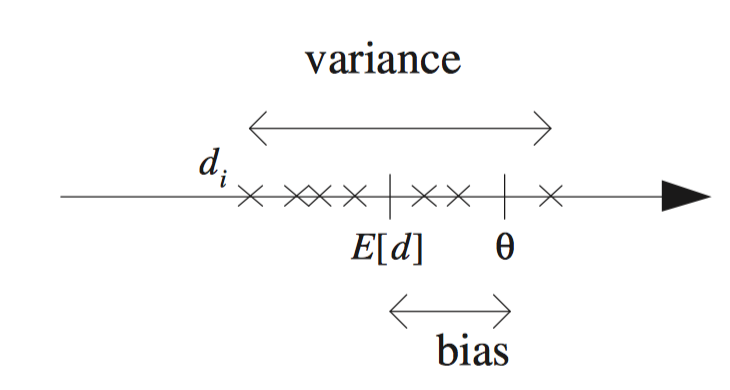
\includegraphics[scale=.6]{images/bias-variance.png}

$\theta$ is the parameter to be estimated. $d_ii$ are several estimates (denoted by '×') over different samples $X_i$ . Bias is the difference between the expected value of $d$ and $\theta$. Variance is how much $d_i$ are scattered around the expected value. We would like both to be small.

\section{Bias of an estimator}
Let $d = d(X)$ be an estimator of $\theta$.

\begin{equation*}
bias_{\theta}(d) = E[d(X)] - \theta
\end{equation*}

If $bias_{\theta}(d)= 0$ for all $\theta$ values, then we say that $d$ is an unbiased estimator of $\theta$.

With $x^t$ drawn from some density with mean $\mu$, $E[\sum_t x^t] = N \mu$.

\section{Variance of an estimator}

\begin{equation*}
variance_{\theta}(d) = E[(d - E[d])^2] 
\end{equation*}

\section{Linear discrimination}
Advantages:
\begin{itemize}
	\item Fast prediction time
	\item Small space to store the prediction function
	\item Knowledge extraction (meaning of weights)
\end{itemize}

Two classes: $g(x) = g_1(x) - g_2(x) = w^T x +w_0$, choose $C_1$ is $g(x)>0$, $C_2$ otherwise.

Multiple classes: Choose $C_i$ is $g_i(x) = max_j g_j(x)$.


$y = P( C_1 | x )$ and $P ( C_2 | x ) = 1 − y$
Choose $C_1$ if $y > 0.5$, which is $y/(1-y) > 1$ or $\log[y/(1-y)] > 0$, $C_2$ otherwise.

Logit: $logit(y) = log[ y/(1-y) ]$ \\
Its inverse is the logistic function, also called sigmoid: $sigmoid(z) = 1/(1+e^{-z})$

\subsection{Logistic regression}
$\log \frac{P(x|C_1)}{P(x|C_2)} = w^T x + w_0'$ \\
$logit(P(C_1|x)) = \log \frac{P(x|C_1)}{1 - P(x|C_1)} = \log \frac{P(x|C_1)}{P(x|C_2)} + \log \frac{P(C_1)}{P(C_2)} = w^T x + w_0$ \\

$y = \frac{1}{1 + e^{-(w^Tx+w_0 )}}$

\subsection{Cross-Entropy error}
$E(w, w_0, | X) = - \sum_t r^t \log y^t + (1 - r^t) \log (1 - y^t)$

We use gradient-descent to minimize the cross-entropy error.

\section{Decision trees}

\textbf{Entropy}: $I = - \sum_i p^{i} \log_2 p^{i}$ where $p^i = \frac{N^i}{N}$
When building the tree, at each node, the algorithm chooses the decision that minimizes: $\sum_{v \in V} \frac{S_v}{S} Entropy(S_v)$

\textbf{Information-Gain}: $Entropy(S) - \sum_{v \in V} \frac{S_v}{S} Entropy(S_v)$

\textbf{Pruning}: 
\begin{itemize}
	\item pre-pruning: early stopping
	\item post-pruning: grow the whole tree then prune subtrees which overfit on the pruning set
\end{itemize}

Pre-pruning is faster, post-pruning is more accurate.


\section{Dimensionality reduction}
Motivation:
\begin{itemize}
	\item Reduce time complexity
	\item Reduce space
	\item Simpler models are more robust on small datasets
	\item More interpretable
\end{itemize}

\textbf{Feature selection}: choose $k<d$ important features

Forward selection: find the best feature one by one and add it iteratively at each step. \\
Backward selection: start with all the features and remove one at a time.

\textbf{Feature extraction}: project the $d$ original features to $k<d$ dimensions (i.e PCA)

PCA is the technique to find a low-dimensional space such that when $x$ is projected there, information loss is minimized.
The core idea is to project the data on the line that produces the highest variance possible.

The projection of $x$ on the direction of $w$ is: $z = w^T x$.

Find $w$ such that $Var(z)$ is maximized.
$Var(z) = Var(w^T x) = E[ (w^Tx -w^T\mu )] = w^T \Sigma w$ where $\Sigma$ is the covariance matrix for $x$.

$\mu = \begin{bmatrix}
	\mu_1 \\	
	\mu_2 \\	
	\dots \\
	\mu_d \\	
\end{bmatrix}
$ is vector of sample means for each column.

Entry in the covariance matrix: $\frac{\sum_t (x_i^t -\mu_i) (x_j^t - \mu_j)}{N-1}$

We want to find $w$ that maximizes $w^T \Sigma w$ such that $||w|| = 1$.
Solution to this problem is Lagrangian multipliers.
$w$ is the eigenvector of $\Sigma$ with the largest eigenvalue.
   
\section{Neural nets}

\subsection{Regression}
$y^t = \sum_h v_h z_h^t + v_0$ \\
$\Delta v_h = \eta \sum_t (r^t - y^t) z_h^t$ \\
$\Delta w_{hj} = -eta \frac{\partial E}{\partial w_{hj}} = - \eta \sum_t \frac{\partial E^t}{\partial y^t} \frac{\partial y^t}{\partial z_h^t}
	\frac{\partial z_h^t}{\partial w_{hj}} = 
	- \eta \sum_t - (r^t -y^t) v_h z_h^t(1-z_h^t)x_j^t = \eta \sum_t (r^t -y^t) v_h z_h^t(1-z_h^t)x_j^t$ \\

The product of the first two terms $(r^t − y^t )v_h$ acts like the error term for hidden unit $h$. This error is backpropagated from the error to the hidden unit. $(r_t - y_t)$ is the error in the output, weighted by the "responsibility" of the hidden unit as given by its weight $v_h$. In the third term, $z_h(1 - z_h)$ is the derivative of the sigmoid and $x_j^t$ is the derivative of the weighted sum with respect to the weight $w_{hj}$.

$E^t(w|x^t, r^t) = \frac{1}{2}(r^t-y^t)^2 = \frac{1}{2}[r^t-(w^tx^t)]^2$

\subsection{Classification}
Single sigmoid output: $y^t = sigmoid(w^Tx^t) = \frac{1}{1 + e^{-w^T x}}$ \\
$E^t(w|x^t, r^t) = -r^t \log y^t - (1-r^t) \log(1-y^t)$ \\
$k > 2$ softmax outputs: $y^t = \frac{e^{w_i^T x^t}}{\sum_k e^{w_k^T x^t}}$ \\
$E^t({w_i}|x^t, r^t) = - \sum_i r_i^t \log y_i^t $

\subsection{Generic update rule}
$\Delta w_{ij}^t = \eta (r_i^t - y_i^t)x_j^t$

\textbf{Batch gradient descent} calculates the error for each example in the training dataset, but only updates the model after all training examples have been evaluated.
    One cycle through the entire training dataset is called a training epoch. Therefore, it is often said that batch gradient descent performs model updates at the end of each training epoch.
    
\begin{itemize}
    \item Fewer updates to the model means this variant of gradient descent is more computationally efficient than stochastic gradient descent
    \item The decreased update frequency results in a more stable error gradient and may result in a more stable convergence
    \item The more stable error gradient may result in premature convergence of the model to a less optimal set of parameters.
    \item The updates at the end of the training epoch require the additional complexity of accumulating prediction errors across all training examples.
    \item 
\end{itemize}

\textbf{Stochastic gradient descent (SGD)}calculates the error and updates the model for each example in the training dataset.
	Stochastic gradient descent is often called an online machine learning algorithm.
\begin{itemize}
	\item The frequent updates immediately give an insight into the performance of the model and the rate of improvement
	\item Simpler to understand and implement
	\item The increased model update frequency can result in faster learning
	\item Updating the model so frequently is more computationally expensive than other configurations of gradient descent, taking significantly longer to train models on large datasets
	\item The frequent updates can result in a noisy gradient signal, which may cause the model parameters and in turn the model error to jump around
\end{itemize}

\subsection{Backpropagation}
\textbf{Chain rule:} $\frac{\partial E}{\partial w_{hj}} = \frac{\partial E}{\partial y_{i}}\frac{\partial y_i}{\partial z_{h}}\frac{\partial z_h}{\partial w_{hj}}$

\textbf{Improving Convergence}
\begin{itemize}
	\item Momentum: is a value between 0 and 1 that increases the size of the steps taken towards the minimum by trying to jump from a local minima.
	    The idea is to take a running average by incorporating the previous update in the current change as if there is a momentum due to previous updates.
		$\Delta w_i^t = - \eta \frac{\partial E^t}{\partial w_i} + \alpha \Delta w_i^{t-1}$
	\item Adaptive learning rate: take smaller and smaller steps as the error decreases.
	$\Delta \eta = \begin{cases}
		+a \text{ if } E^{t+\tau} < E^t \\
		-b\eta \text{ otherwise}
	\end{cases}$
\end{itemize}

\section{Clustering}

Unsupervised learning problem.

$Error = \sum_t || x^{(t)} - e(x^{(t)}) ||$ where $e(x^{(t)})$ cluster representative for $x^{(t)}$.
Centroid is the mean of the cluster, defined as $m_i = \frac{\sum_{x \in C_i} x}{|C_i|}$
\subsection{k-means clustering}
Every cluster has a representative. Each example is assigned to the cluster having closest representative.
Closeness can be measured using Euclidean distance.
$||x-y||=\sqrt{\sum_{i=1}^d (x_i - y_i)^2}$

Error is defined as $\sum_t || x^{(t)} - \rho(x^{(t)})||^2$ where $\rho(x^{(t)})$ is representative of $x^{(t)}$

How to handle empty cluster:
\begin{itemize}
	\item choose the closest point in the dataset to the previous representative of the empty cluster
	\item restart with new cluster representative
	\item continue with remaining $k' < k$ clusters 
	\item assign a new cluster representative to the point with highest squared error
\end{itemize}

\textbf{Soft clustering}: points are not assigned to a cluster, but the have probabilities of being in a clusters.

\textbf{Clustering for concentric data}: concentric circles would have the exact same mean, so k-means is not suitable to separate them. If you know that your clusters will always be concentric circles, you can simply convert your cartesian (x-y) coordinates to polar coordinates, and use only the radius rho for clustering 


\subsection{Expectation-Maximization for mixture of Gaussians}
$E[z^{(j)} | x ] = p(z^{(j)} | x) = \frac{p(x|z^{(j)}) p(z^{(j)})}{p(x)} = \frac{p(x|z^{(j)})}{\sum_j p(x|z^{(j)})}$ \\
$\mu^{(j)} = \frac{\sum_x x \cdot p(z{(j)} | x )}{\sum_x p(z^{(j)} | x)}$ \\

$\log p(D|h) = \sum_i \log [p(x^{(i)} | z^{(1)})\frac{1}{2} +  p(x^{(i)} | z^{(2)})\frac{1}{2}]$



\section{SVMs}
\subsection{Maximum margin hyperplane}
The hyperplane that maximizes margin. Margin is the distance from the hyperplane to the closest training example. Margin is equal to $\frac{1}{||w||}$ for the support vectors.

$
\begin{cases}
	w^T x^{(t)} + w_0 \geq 1$ if $x^{(t)} = +1 \\ 
	w^T x^{(t)} + w_0 \leq 1$ if $x^{(t)} = -1
\end{cases}
$

Maximizing margin is the same as minimizing $||w||$ (or $||w||^2$)

$r = \frac{g(x)}{||w||}$, if $g(x) = a x_1 + b x_2 + c = 0$ then $||w|| = \sqrt{a^2 +b^2}$

Large numbers of support vector are an indication that overfitting might be occurring.
High penalty parameter $\lambda$ increases the danger of overfitting.

A good practice when training SVM is to normalize or standardize the attribute values. 

When data is not linearly separable we use mapping to map to a new dimension where it is linearly separable. 

\subsection{Kernel functions}

\textbf{Polynomial kernel} Given $\phi(x): [1, \sqrt x_1, \sqrt x_2, \sqrt{x_1x_2}, x_1^2, x_2^2 ]$,
so $K(x, y) = \phi(x) \cdot \phi(y) = (1 + x_1 y_1 + x_2 y_2)^2 = (1 + x \cdot y)^2$.
For $d$ dimensions: $K(x, y) =(1 + x \cdot y)^d$

\textbf{Gaussian (RBF) kernel} is $K(x, y) = e^{-\frac{||x-y||^2}{\sigma^2}}$

The smaller the value of $\sigma$, the smaller the width of the Gaussian around the support vectors. This is likely to result in test points being classified according to the label of the closest support vector.
\subsection{Soft-margin SVM}
It can be used when data is not linearly separable. Suppose have separating hyperplane with some exception, as few points with smaller margin or in the wrong side of the hyperplane.

We introduce a slack variable $\xi^{(i)}$ for every training example $x^{(i)}$, where $\xi^{(i)} \geq 0$. 

Now we want to satisfy $w^T x^{(i)} + w_0 + \xi^{(i)} \geq 1$. 

So now we minimize $\frac{1}{2} ||w||^2 + \lambda \sum_i \xi^{(i)}$


\subsection{Advantages \& disadvantages of SVMs}
Advantage: Kernels allow you to do well with complex data. 
Disadvantages: slow training, difficulty in understanding how to method worked (w\ Gaussian kernel, results depend heavily on settings of tunable parameters like $\sigma$ and the choice of kernel.
 
\section{Ensemble methods}
Since there is no single learning algorithm that in any domain always induces the most accurate learner, by suitably combining multiple base-learners then, accuracy can be improved.

\section{Bagging}
Bagging is a voting method whereby base-learners are made different by training them over slightly different training sets.
Generating $L$ slightly different samples from a given sample is done by bootstrap, where given a training set $X$ of size $N$, we draw $N$ instances randomly from $X$ with replacement. Because sampling is done with replacement, it is possible that some instances are drawn more than once and that certain instances are not drawn at all. When this is done to generate $L$ samples, these samples are similar because they are all drawn from the same original sample, but they are also slightly different due to chance.

\section{Boosting}
In boosting, we actively try to generate complementary base-learners by training the next learner on the mistakes of the previous learners.

\section{Appendix}
\subsection{Transpose of a matrix}
Switch the row and column indices of the matrix.

$A =\begin{bmatrix}
    a_{1,1} & a_{1,2} & \dots & a_{1,j} \\
    a_{2,1} & a_{2,2} & \dots & a_{2,j} \\
    \dots & \dots & \dots  &\dots        \\
    a_{i,1} & a_{i,2} & \dots & a_{i,j} \\
\end{bmatrix}$  $A^T =\begin{bmatrix}
    a_{1,1} & a_{2,1} & \dots & a_{i,1} \\
    a_{1,2} & a_{2,2} & \dots & a_{i, 2} \\
    \dots & \dots & \dots  &\dots        \\
    a_{1,j} & a_{2, j} & \dots & a_{i, j} \\
\end{bmatrix}$

\subsection{Inverse of a matrix}
$\begin{bmatrix}
    a_{1,1} & a_{1,2} \\
    a_{2,1} & a_{2,2} \\
\end{bmatrix} ^{-1} = 
\frac{1}{a_{1,1} a_{2,2} - a_{1,2} a_{2,1}}
\begin{bmatrix}
	a_{2,2} & -a_{1,2} \\
    -a_{2,1} & a_{1,1} \\
\end{bmatrix}
$ \\
Generic matrix\\
$A = \begin{bmatrix}
    a_{1,1} & a_{1,2} & a_{1,3} \\
    a_{2,1} & a_{2,2} & a_{2,3} \\
    a_{3,1} & a_{3,2} & a_{3,3} \\
\end{bmatrix}$ \\ 

Calculate the "Matrix of Minors".\\
$A' = \begin{bmatrix}
    a_{1,1}' & a_{1,2}' & a_{1,3}' \\
    a_{2,1}' & a_{2,2}' & a_{2,3}' \\
    a_{3,1}' & a_{3,2}' & a_{3,3}' \\
\end{bmatrix}$\\

$a_{1,1}' = \begin{bmatrix}
    \bullet &  &  \\
    	 & a_{2,2} & a_{2,3} \\
    	 & a_{3,2} & a_{3,3} \\
\end{bmatrix} = a_{2,2} a_{3,3} - a_{2,3}a_{3,2}$

Apply a "checkerboard" of minuses to the "Matrix of Minors" and obtain the "Matrix of Cofactors". \\
$A' \rightarrow \begin{bmatrix}
    + & - & + \\
    - & + & - \\
    + & - & + \\
\end{bmatrix} \rightarrow A''$

Transpose the "Matrix of Cofactors"(Adjugate)

Multiply by 1/Determinant of the original matrix
$A^{-1} = \frac{1}{det(A)} (A'')^T$
\\

\subsection{FPR and TPR}
$FPR = FP/(TN + FP)$\\
$TPR = TP/(TP + FN)$

\subsection{Eigenvalues and Eigenvectors}
The characteristic polynomial of a matrix A is given by $|A - \lambda I|$. 
We solve $det(A - \lambda I) = 0$ to find the eigenvalues. 

For each eigenvalue $k$, to find the eigenvectors we look for the solution $v$ of the homogeneous system of equations $(A - k I)v=0$. This will produce a system of equations, whose solution is the eigenvector for the given eigenvalue.

\subsection{Conditional entropy}
\resizebox{.9 \textwidth/3}{!} 
{
 $H(Y|X) = \sum_x P[X=x] \cdot (\sum_y -P[Y=y | X=x] \cdot \log_2 P[Y=y|X=x])$
}

\smallskip
\rule{0.3\linewidth}{0.25pt}
\scriptsize

Copyright \copyright\ 2018 Antonio Mallia

\href{https://www.antoniomallia.it}{https://www.antoniomallia.it}

\end{multicols}
\end{document}
